\section{Empirical Evaluation}
  
In this section we compare the solutions for traffic networks modeled as a QTM
using homogeneous and non-homogeneous time intervals in two aspects:
%
the quality of the solution and convergence to the \remark{optimal
solution}.\fnremark{FWT: I don't think that optimal is the best word here since
we arbitrarily fixed a value of \DT[]. Also, there is the technical problem that
Gurobi might not have found the true optimal.}
%
We compare the quality of solutions based on the total travel time and we also
consider the third quartile and maximum of the observed delay distribution.
%
%% TODO(fwt): maybe define what we mean by optimal here, for instance
%
%For our experiments, we consider as optimal solution, the MILP solution of a
%QTM using small enough homogeneous \DT[] with unlimited computational
%resources.
%
Our hypotheses are:
%
(i) the quality of the non-homogeneous solutions is at least as good as the
homogeneous ones when the number of time intervals~\Nn is fixed; and 
%
(ii) the non-homogeneous approach requires less time intervals (i.e., smaller
\Nn) than the homogeneous approach to converge to the optimal solution.
%
In the remainder of this section, we present the traffic networks considered in
the experiments, our methodology, and the results.



\subsection{Networks}

We consider three networks of increasing complexity: an avenue crossed by three
side streets; a 2-by-3 grid; and a 3-by-3 grid with a diagonal avenue.
%
The queues receiving cars from outside of the network are marked in
\cref{fig:networks} and we refer to them as input queues.
%
The maximum capacity~(\QMAX{i}) is 60 cars for non-input queues and
\remark{infinity} for input queues to prevent interruption of the input demand
due to spill back from the stop line. 
%
The traversal time of each queue $i$~(\QDELAY{i}) is set at 9s (a distance of
about 100m with a free flow speed of 50km/h).
%
Flows are defined from the head of each queue $i$ into the tail of the next
queue $j$;
%
there is no turning traffic ($\FTURN{i}{j}=1$), and the maximum flow rate
between queues, \FMAX{i}{j}, is set at 5 cars/s.
%
All traffic lights have two phases, north-south and east-west, and lights 2, 4
and 6 of network 3 have the additional northeast-southwest phase to control the
diagonal avenue.
%
For networks 1 and 2, \PTMIN{\tl}{k} is 1s, \PTMAX{\tl}{k} is 3s, \CTMIN{\tl} is
2s, and \CTMAX{\tl} is 6s, for all traffic light \tl and phase $k$.
%
For network 3, \PTMIN{\tl}{k} is 1s and \PTMAX{\tl}{k} is 6s for all \tl and
$k$; and \CTMIN{\tl} is 2s and \CTMAX{\tl} is 12s for all lights \tl except for
lights 2, 4 and 6 in which \CTMIN{\tl} is 3s and \CTMAX{\tl} is 18s.




\subsection{Experimental Methodology}

%\begin{table}[h]
%\caption{Network Demand Profiles (vehicles per second)}
%\label{tab:network_demand}
%\centering
%\begin{tabular}{cccccc}
%\toprule
%& Inflow Queues & 0 - 55 s & 55 - 70 s & 70 - 85 s & > 85 s\\
%\midrule
%\multirow{2}{*}{Network 1}&$q_0$ & 1 & 1 & 1 & 0 \\
%&$q_4, q_7$ & 4 & 4 & 4 & 0 \\
%&$q_1,q_{10}$& 2 & 4 & 2 & 0 \\
%\midrule
%\multirow{2}{*}{Network 2}&$q_0$ & 1 & 1 & 1 & 0 \\
%&$q_4,q_7,q_{14}$& 4 & 4 & 4 & 0 \\
%&$q_1, q_{10},q_{18}$ & 2 & 4 & 2 & 0 \\
%\midrule
%\multirow{2}{*}{Network 3}&$q_0$ & 1 & 1 & 1 & 0 \\
%&$q_4,q_7,q_{14},q_{25},$& 4 & 4 & 4 & 0 \\
%&$q_1, q_{10},q_{18},q_{29},q_{36},q_{40},q_{44}$ & 2 & 4 & 2 & 0 \\
%\bottomrule\\
%\end{tabular}
%\end{table}


For each network, a constant background level traffic is injected in the network
in the first 55s to allow the solver to settle on a stable policy.
%
Then a spike in demand is introduced in the queues marked as \qVarTraf from time
55s to 70s to trigger a policy change.
%
%with the expectation that plans generated with longer look ahead will produce a
%more coordinated global policy change.
%
From time 70s to 85s, the demand is returned to the background level, and then
reduced to zero for all input queues.
%
We extend the problem horizon~\TMAX until all cars have left the network.
%
By clearing the network, we can easily measure the total travel time for all the
traffic as the area between the cumulative arrival and departure curves measured
at the boundaries of the network.\fnremark{FWT: is this explanation of how to
compute the total travel time still necessary?}
%
%\cref{tab:network_demand} presents the demand profile of each network.
%
The background level for the input queues are 1, 4 and 2 cars/s for queues
marked as \qLowTraf, \qHighTraf and \qVarTraf, respectively; and during the high
demand period, the queues \qVarTraf receive 4 cars/s.



% def major and minor frame tell about overlapping and fig:multiplan show
% parameters, i.e., delta ts
% - fairness: same delta t for minor frame
For both homogeneous and non-homogeneous intervals, we use the MILP QTM
formulation~(\cref{sec:milp}) in a receding horizon manner: a control plan is
computed for a pre-defined horizon (smaller than \TMAX) and only a prefix of
this plan is executed before generating a new control plan. 
%
\cref{fig:multiplan} depicts our receding horizon approach and we refer to the
planning horizon as a major frame and its executable prefix as a minor frame.
%
Notice that, while the plan for a minor frame is being executed, we can start
computing the solution for the next major frame \remark{based on a forecast
model}.\footnote{FWT: not sure if we should mention this.}


To perform a fair comparison between the homogeneous and non-homogeneous
discretizations, we fix the size of all minor frames to 10s and force it to be
discretized in homogeneous intervals of 0.25s.
%
For the homogeneous experiments, \DT[] is kept at 0.25s throughout the major
frame; therefore, given \Nn, the major frame size equals $\Nn/4$ seconds for the
homogeneous approach.
%
For the non-homogeneous experiments, \DT[] linearly increases from
0.25s at the end of the minor frame to 1.0s at the end of the major frame;
therefore, the major frame size used by the non-homogeneous approach
is $10.375 + 0.625(\Nn-40)$ seconds for a given $\Nn > 40$.\toIain{Double check
this.}
%
%We analyze the effect of the major frame size by varying it from 20s through to 
%120s.
%
% explain evaluation: concatenation + LP simulation Overall ``optimal'' for
% comparison
Once we have generated a series of minor frames, we concatenate them into a
single plan and simulate the flow through the network using the QTM LP
formulation with a fixed (homogeneous) $\DT[]$ of 0.25s.
%
\fnremark{Do we need to justify why we use the QTM as the simulator over say a
micro simulator?}
%
We also compare both receding horizon approaches against the \remark{optimal}
solution obtained by computing a single control plan for the entire control
horizon (i.e., $[0,\TMAX]$) using a fixed \DT[] of 0.25s.


For all our experiments, we used Gurobi\textsuperscript{TM} as MILP solver with
12 threads on a 3.1GHz AMD Opteron\textsuperscript{TM}~4334 processor with 12
cores.
%
We limit MIP gap accuracy to 0.1\% and the time cutoff for solving a major frame
to 3000s for the receding horizon approaches and unbounded for the optimal plan.
%
%% \toIain{Can you explain the following better and provide evidence:
%% \textit{while we can solve non-homogeneous major frames up to convergence in
%% real time, we extend the solve time limit to 3000s for all test points for a
%% fair comparison with the homogeneous test points.}?
%%
%% Iain: Deleted as it was not strictly true. Either we re-run scaled up on AWS
%% with 10s solver time limit. Or we perhaps explain that 3000s shows that it
%% could be scaled up to real time}
%
All our results are averaged over five runs \remark{to account for Gubori's
stochastic strategies.}


\begin{figure*}[t!]
\centering
%  trim={<left> <lower> <right> <upper>}
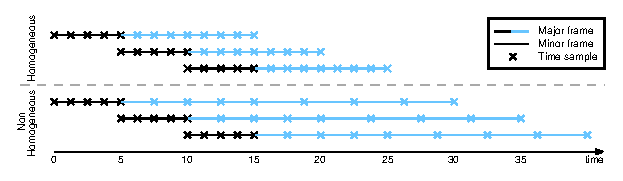
\includegraphics[width=1.0\textwidth]{non_homogeneous_control.eps}
\caption{Receding horizon planning}
\label{fig:multiplan}
\end{figure*}


\begin{figure*}[t!]
\centering
%  trim={<left> <lower> <right> <upper>}
\subfigure[]{
\label{subfig:network1}
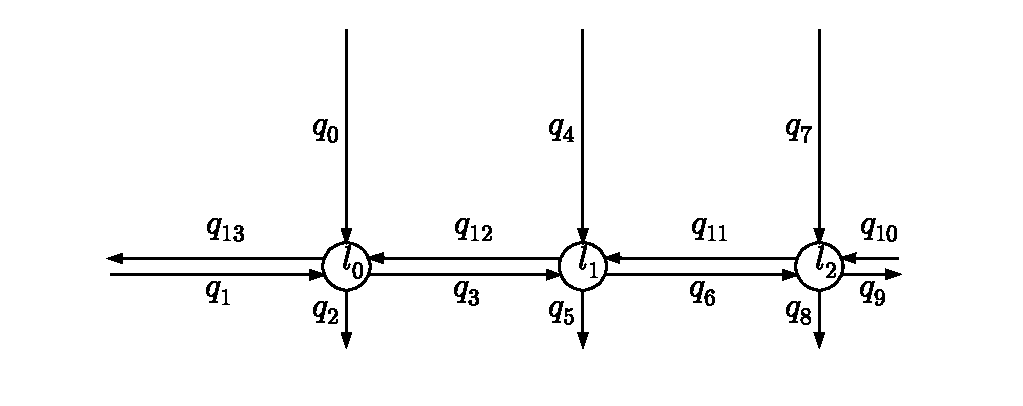
\includegraphics[width=0.45\textwidth]{network_3_lights}}
\subfigure[]{
\label{subfig:network2}
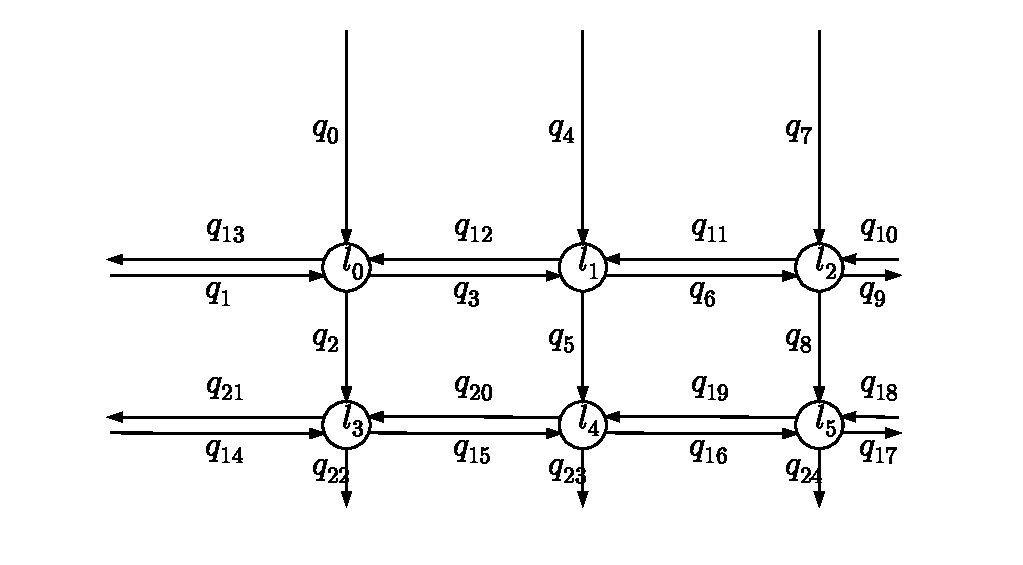
\includegraphics[width=0.45\textwidth]{network_6_lights}}
\subfigure[]{
\label{subfig:network3}
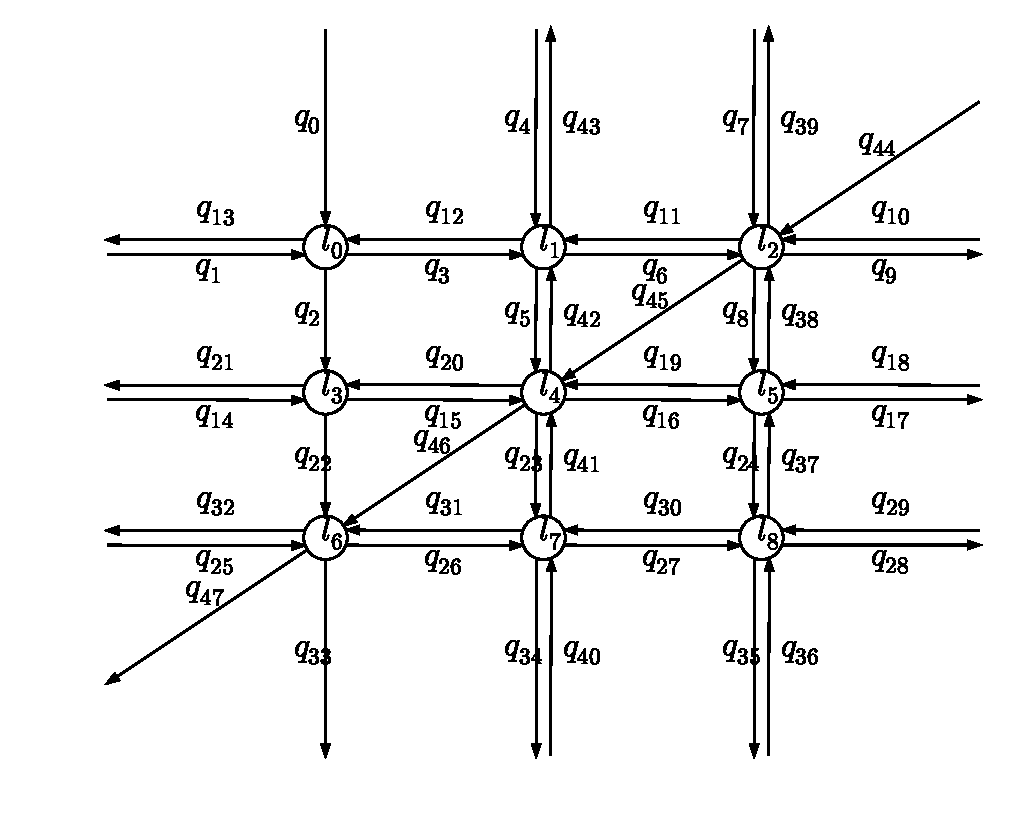
\includegraphics[width=0.45\textwidth]{network_9_lights}}
\caption{Networks used to evaluate the QTM performance. \remark{Iain: please,
mark the input queues.}}
\label{fig:networks}
\end{figure*}




%\begin{table}[h]
%\caption{Network 3 traffic parameters}
%\label{tab:net3wave}
%\centering
%\begin{tabular}{cccccc}
%\toprule
%Queue & Background & End & Wave & Start &End\\ 
%\midrule
%$q_0$ & 1 & 85 & 1 & 55 & 70\\
%$q_1$ & 2 & 85 & 4 & 55 & 70\\
%$q_4$ & 4 & 85 & 4 & 55 & 70\\
%$q_7$ & 4 & 85 & 4 & 55 & 70\\
%$q_{10}$ & 2 & 85 & 4 & 55 & 70\\
%$q_{14}$ & 4 & 85 & 4 & 55 & 70\\
%$q_{18}$ & 2 & 85 & 4 & 55 & 70\\
%$q_{25}$ & 4 & 85 & 4 & 55 & 70\\
%$q_{29}$ & 2 & 85 & 4 & 55 & 70\\
%$q_{36}$ & 2 & 85 & 4 & 55 & 70\\
%$q_{40}$ & 2 & 85 & 4 & 55 & 70\\
%$q_{44}$ & 2 & 85 & 4 & 55 & 70\\
%\bottomrule\\
%\end{tabular}
%\end{table}


\subsection{Results}

%We compare the performance of non-homogeneous and homogeneous solutions in two
%ways: comparing the decrease in total travel time with increasing major frame
%time (greater look ahead), and analysing the distribution of delay in each
%queue of the network.
%
\cref{subfig:travel_time_3,subfig:travel_time_6,subfig:travel_time_9} show, for
each network, the increase in the total travel time w.r.t. the optimal solution
as a function of \Nn.
%
As we hypothesized, the non-homogeneous discretization requires less time
intervals to converge.
%
This is important because the size of the MILP, including the number of binary
variables, scales linearly with \Nn; therefore, the non-homogeneous approach can
scale up better than the homogeneous one (e.g., \cref{subfig:travel_time_9}).


The distribution of the total delay observed by each car while traversing the
network is shown in \cref{subfig:delay_3,subfig:delay_6,subfig:delay_9}.
%
Each group of box plots represents a different value of \Nn: when the
non-homogeneous $\DT[]$ first converges to the optimum solution; when the
homogeneous $\DT[]$ first converges on the optimum solution; and the optimum
solution itself.
%
In all networks, the quality of the solution obtained using non-homogeneous
$\DT[]$ is better or equal than using homogeneous $\DT[]$ for fixed \Nn in both
the total travel time and \emph{fairness}, i.e., smaller third quartile and
maximum delay.

\remark{FWT: In the paragraphs above, we need to address network 2 because it is
the exception in both cases: in the end of \cref{subfig:travel_time_6},
homogeneous is better, and the homogeneous delay in \cref{subfig:delay_6} is
also better.}


Finally, \cref{fig:cumu} shows the cumulative arrival and departure curves and
the how delay evolves over time for $q_1$ of network 2.  \cref{subfig:cumu1}
shows the comparison at the point where the non-homogeneous $\DT[]$ first
converges and shows that with the longer major frame time of the
non-homogeneous $\DT[]$, the solver is able to find a coordinated signal policy
along the avenue to dissipate the extra traffic that arrives at the 55s point,
while the homogeneous $\DT[]$ with its shorter major frame \remark{fails to find
a coordinated policy along the avenue and experiences more delay}.\toIain{I
don't think that failure to coordinate is the best way to describe it because
there is coordination but it happens too late.} Once the homogeneous $\DT[]$ has
converged in \cref{subfig:cumu2}, both solutions are close to the optimum
solution which is shown in \cref{subfig:cumu3}.\fnremark{FWT: although
\cref{fig:cumu} is a nice illustration of how homogeneous and non-homogeneous
differ, it is currently not backing up any of our claims.}


\begin{figure*}[t!]
\centering

%  trim={<left> <lower> <right> <upper>}
\subfigure[]{
\label{subfig:travel_time_3}
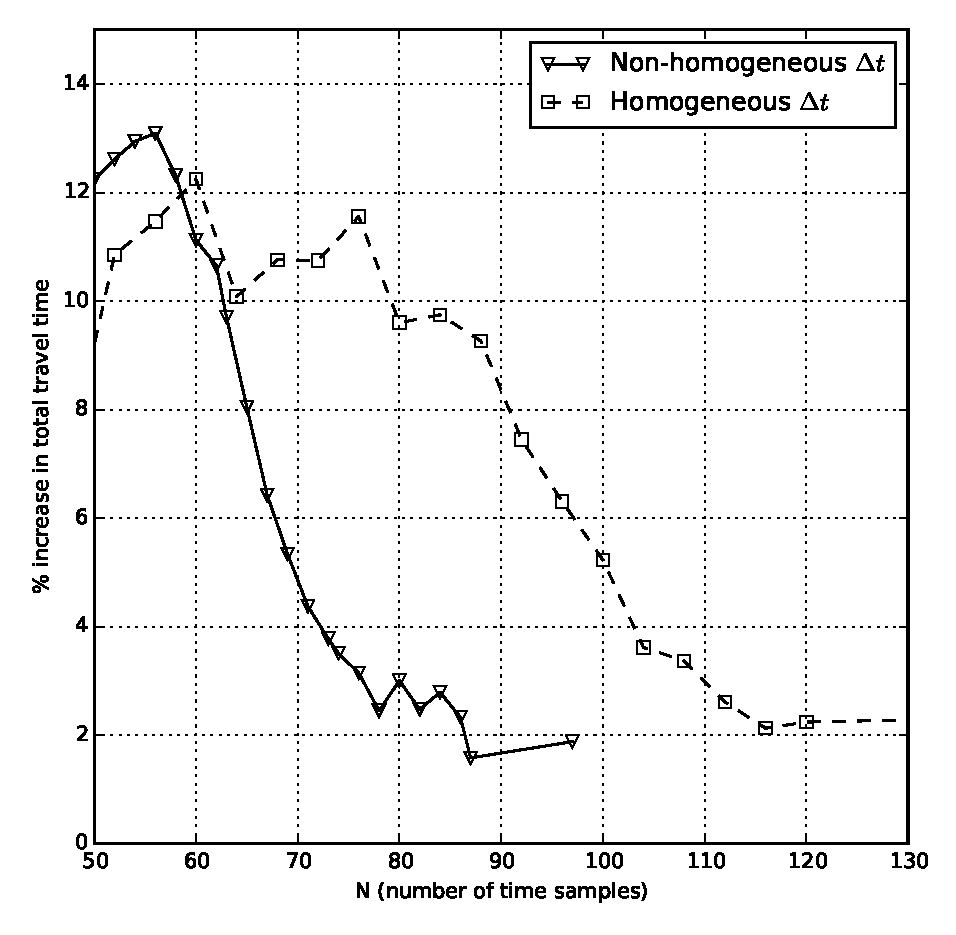
\includegraphics[keepaspectratio,height=0.31\textwidth]{samples_plot_3_lights}}
\subfigure[]{
\label{subfig:delay_3}
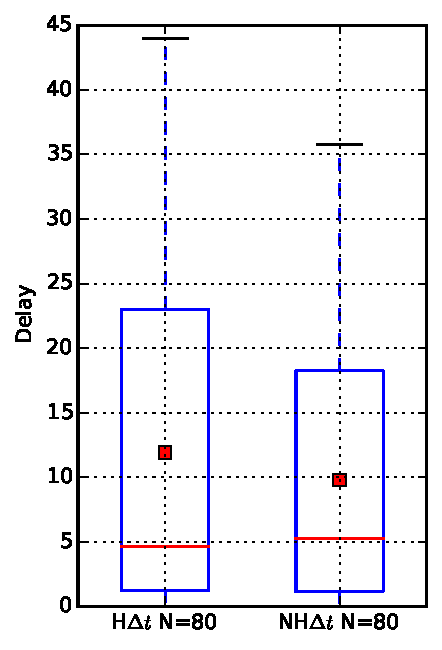
\includegraphics[keepaspectratio,height=0.31\textwidth]{box_plot_early_3l.pdf}
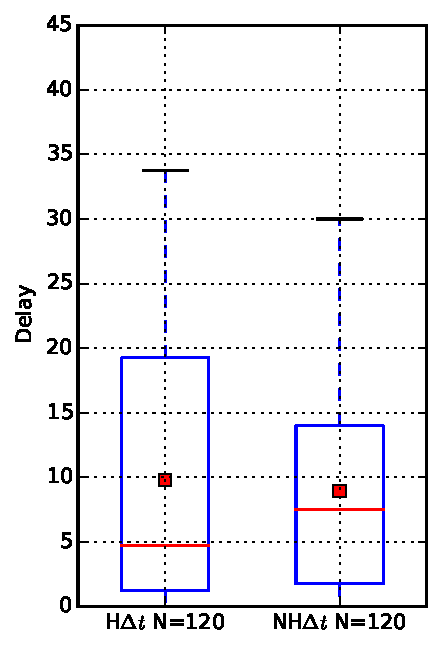
\includegraphics[keepaspectratio,height=0.31\textwidth]
{box_plot_converg_3l.pdf}
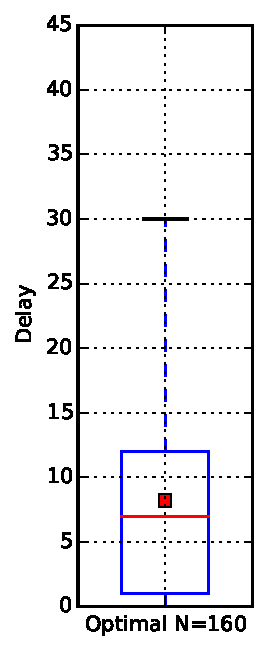
\includegraphics[keepaspectratio,height=0.31\textwidth]{box_plot_final_3l.pdf}}

\subfigure[]{
\label{subfig:travel_time_6}
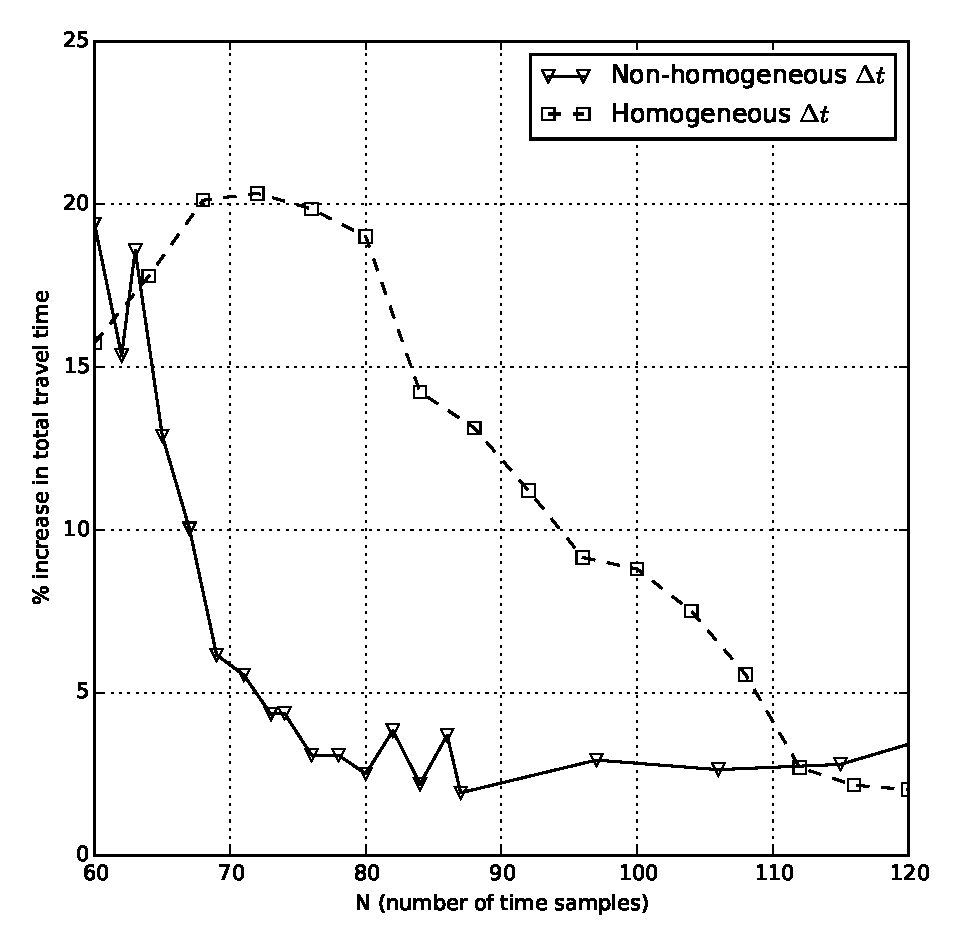
\includegraphics[keepaspectratio,height=0.31\textwidth]{samples_plot_6_lights}}
\subfigure[]{
\label{subfig:delay_6}
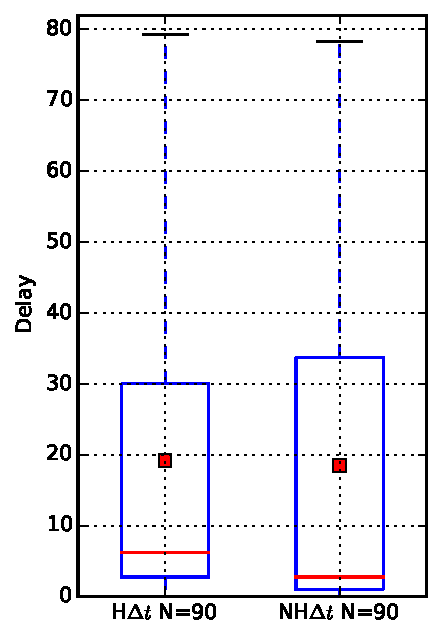
\includegraphics[keepaspectratio,height=0.31\textwidth]{box_plot_early_6l.pdf}
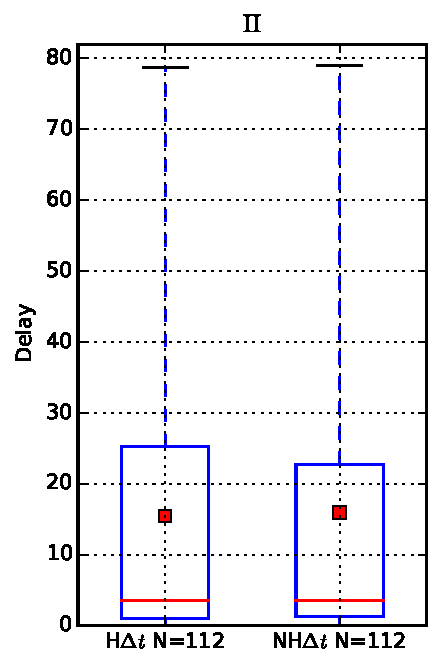
\includegraphics[keepaspectratio,height=0.31\textwidth]
{box_plot_converg_6l.pdf}
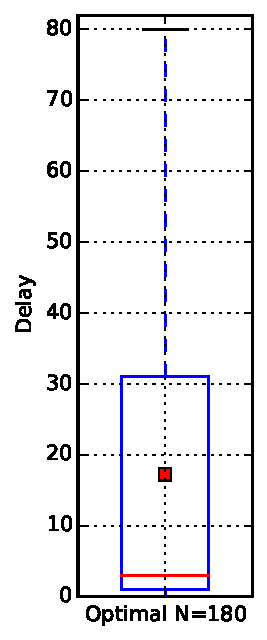
\includegraphics[keepaspectratio,height=0.31\textwidth]{box_plot_final_6l.pdf}}

\subfigure[]{
\label{subfig:travel_time_9}
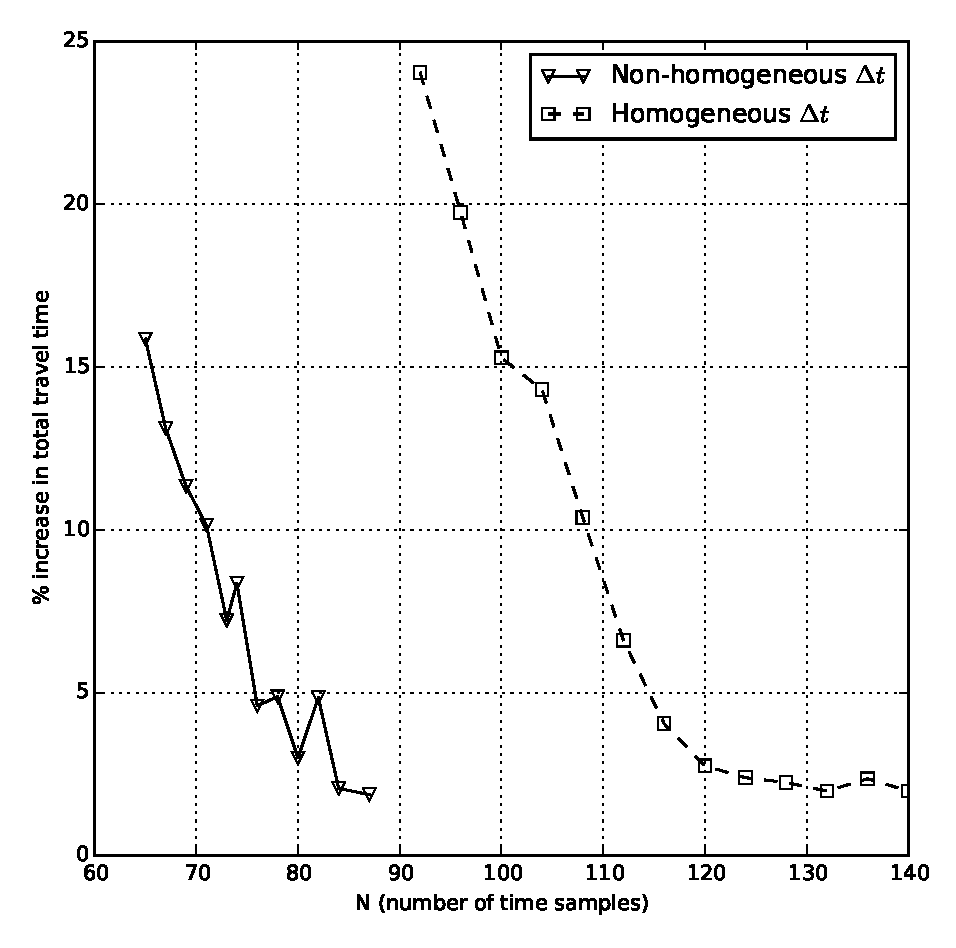
\includegraphics[keepaspectratio,height=0.31\textwidth]{samples_plot_9_lights}}
\subfigure[]{
\label{subfig:delay_9}
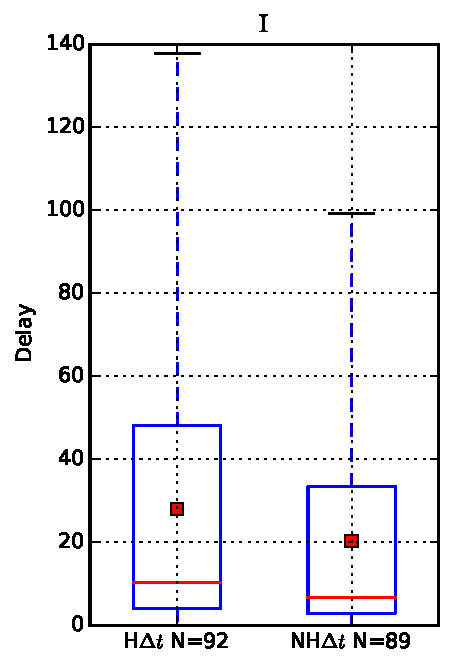
\includegraphics[keepaspectratio,height=0.31\textwidth]{box_plot_early_9l.pdf}
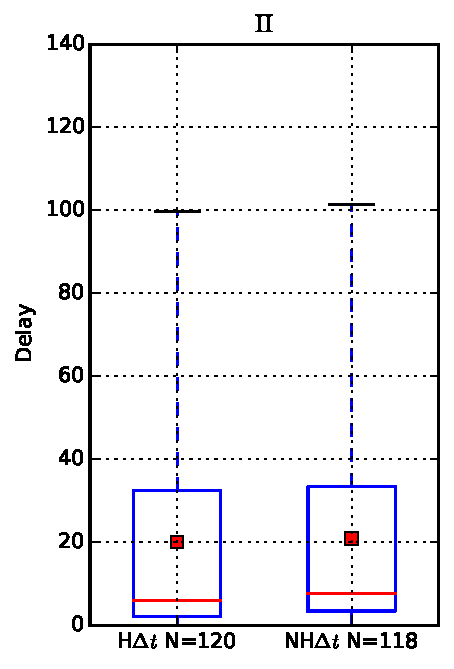
\includegraphics[keepaspectratio,height=0.31\textwidth]
{box_plot_converg_9l.pdf}
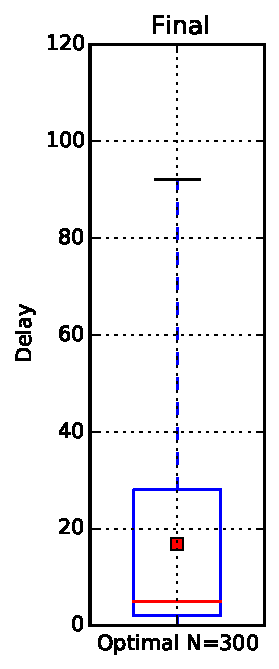
\includegraphics[keepaspectratio,height=0.31\textwidth]{box_plot_final_9l.pdf}}
\caption{Results for the three networks showing the comparitive \% increase in 
total travel time for the network between using a homogeneous $\DT[]$ and a 
non-homogeneous $\DT[]$, and the 
distribution of delay time at the convergence point of non-homogeneous $\DT[]
$, the convergence point of homogeneous $\DT[]$ and for the fully solved 
optimal solution. (a) and (b) 3 light avenue, 
(c) and (d) 6 light grid, and (e) and (f) 9 light grid.}
\label{fig:results}
\end{figure*}

\begin{figure*}[t!]
\centering

%  trim={<left> <lower> <right> <upper>}
\subfigure[]{
\label{subfig:cumu1}
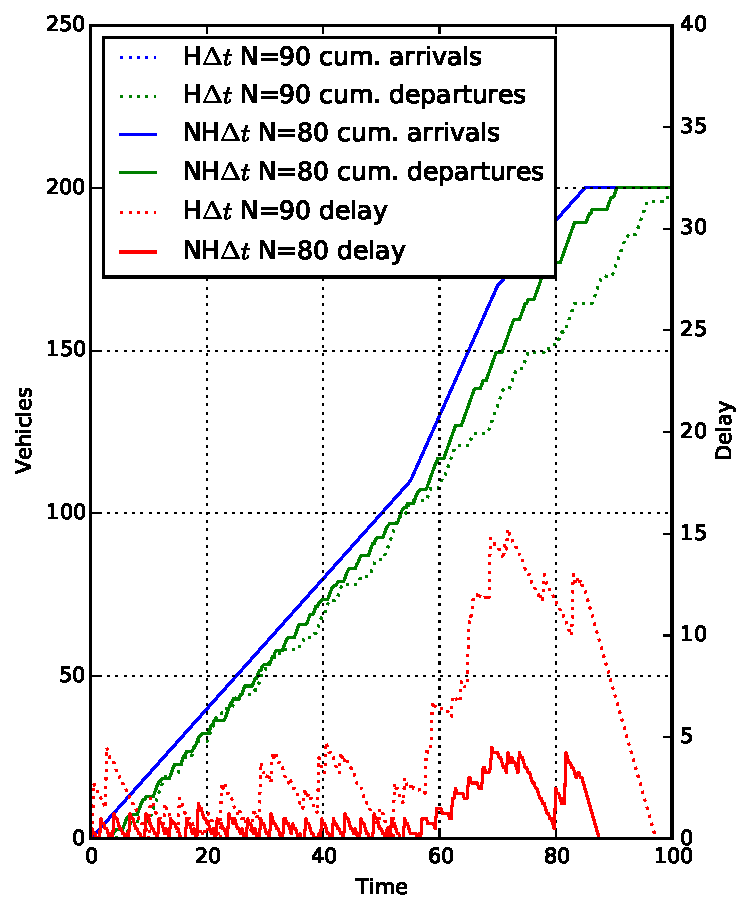
\includegraphics[width=0.32\textwidth]{cum_plot_early_6l.pdf}}
\subfigure[]{
\label{subfig:cumu2}
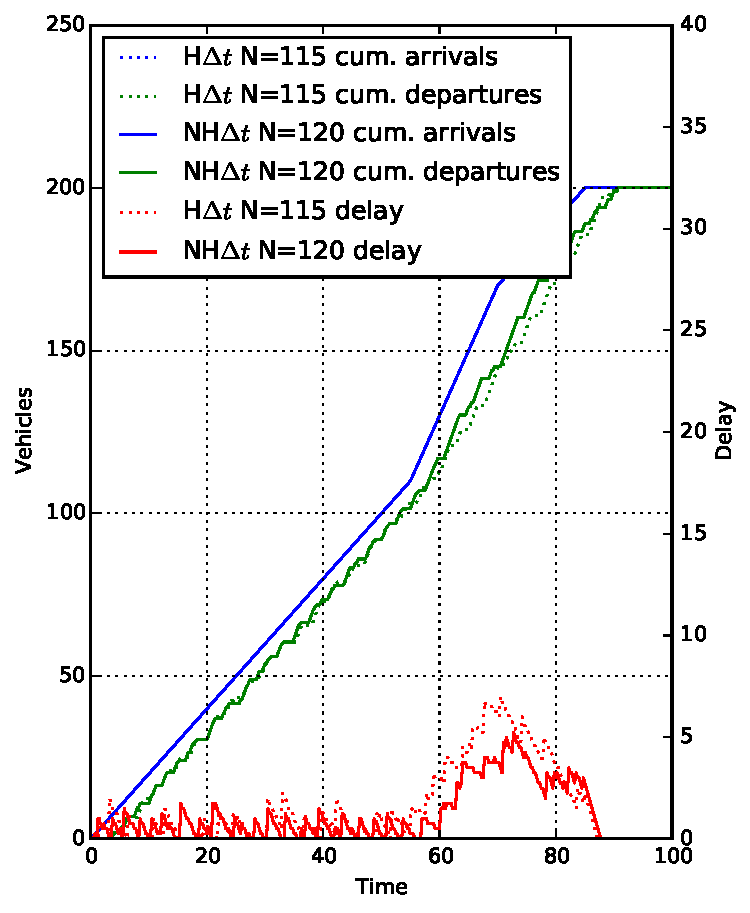
\includegraphics[width=0.32\textwidth]{cum_plot_converg_6l.pdf}}
\subfigure[]{
\label{subfig:cumu3}
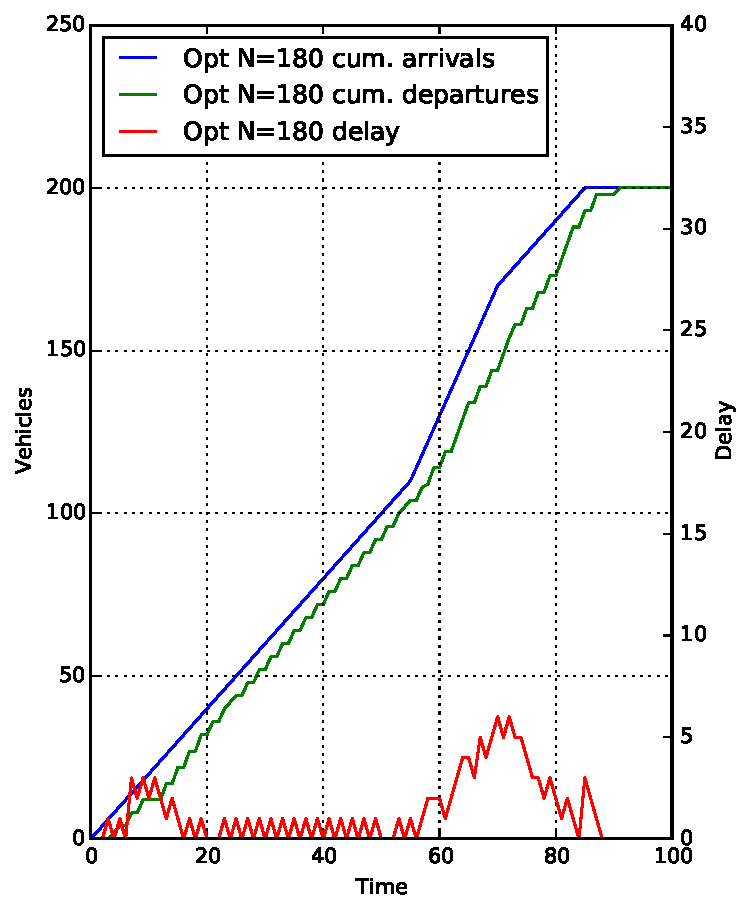
\includegraphics[width=0.32\textwidth]{cum_plot_final_6l.pdf}}
\caption{Cumulative arrival and departure curves and delay for queue 1 in the 6 
light grid. (a) at the convergence point of the non-homogeneous $\DT[]$ it is 
near to the optimum solution while 
homogeneous $\DT[]$ lags behind (b) at the convergence point of 
homogeneous $\DT[]$ both are near optimum, and (c) the fully solved optimal 
solution}
\label{fig:cumu}
\end{figure*}

